% This text is proprietary.
% It's a part of presentation made by myself.
% It may not used commercial.
% The noncommercial use such as private and study is free
% Sep. 2005 
% Author: Sascha Frank 
% University Freiburg 
% www.informatik.uni-freiburg.de/~frank/


\documentclass{beamer}
\mode<presentation>
{
  \usetheme{Madrid}       % or try default, Darmstadt, Warsaw, ...
  \usecolortheme{default} % or try albatross, beaver, crane, ...
  \usefonttheme{serif}    % or try default, structurebold, ...
  \setbeamertemplate{navigation symbols}{}
  \setbeamertemplate{caption}[numbered]
}

\AtBeginSection[]
{
\setbeamercolor{section in toc}{fg=alerted text.fg}
\setbeamercolor{section in toc shaded}{fg=structure}
\begin{frame}<beamer>
  \frametitle{Outline}
  \tableofcontents[currentsection]
\end{frame}
}

\usepackage[french]{babel}
\usepackage[utf8x]{inputenc}

\title{Atelier musique libre}   
\author{Louvain-li-Nux}

\begin{document}

\frame{\titlepage}

\begin{frame}{Table des matières}
  \tableofcontents
\end{frame}

%%% INTRODUCTION %%%
\section{Introduction}
\begin{frame}{Introduction}
\end{frame}

\subsection{La MAO, qu'est-ce que c'est ?}
\begin{frame}{La MAO, qu'est-ce que c'est ?}
  \textbf{MAO} (musique assistée par ordinateur) = \textit{l'ensemble des utilisations de \textbf{l'informatique} comme outil pour la \textbf{création}, la \textbf{diffusion} et la formation \textbf{musicale}.}
  Cela comprend :
  \begin{itemize}
  \item la composition : séquençage MIDI, boucles musicales, ... ;
  \item l'édition de partitions ;
  \item la lecture de son et la synthèse sonore ;
  \item l'enregistrement audio ;
  \item l'édition audio ;
  \item le traitement du son ;
  \item la conversion et la diffusion ;
  \item et plus encore.
  \end{itemize}
\end{frame}

\begin{frame}{Comment faire de la MAO ?}
  Aspect \textbf{matériel} :
  \begin{itemize}
  \item ordinateur ;
  \item interface audio (carte son) ;
  \item enceintes de monitoring ;
  \item instruments, interfaces MIDI, micros.
  \end{itemize}
  \vskip1em
  
  Aspect \textbf{logiciel} :
  \begin{itemize}
  \item Windows, Mac ou \textbf{Linux} ;
  \item logiciel d'enregistrement et de montage ;
  \item séquenceur MIDI ;
  \item sampler/échantillonneur et synthétiseur ;
  \item plugins, effets, ...
  \end{itemize}
\end{frame}



\subsection{Pourquoi des logiciels libres ?}
\begin{frame}{Différence entre libre et propriétaire}
  %TODO: c'est une parenthèse que je pense utile.
\end{frame}

\begin{frame}{Pourquoi des logiciels libres ?}
  Il existe beaucoup de solutions propriétaires pour faire de la MAO. On peut citer par exemple Cubase, Pro Tools, FL Studio, Garage Band. Ces logiciels sont très bons et largement utilisés dans le milieu professionnel.
  \vskip1em
  
  \textbf{Quels sont les intérêts des logiciels libres ?}
  \begin{itemize}
  \item Prix
  \item Qualité
  \item Communauté
  \item Diversité
  \end{itemize}
\end{frame}

\begin{frame}{Pourquoi des logiciels libres ?}
  \begin{itemize}
  \item \textbf{Prix}
  
    Même si libre $\neq$ gratuit, c'est souvent le cas.
    
    Tous les logiciels utilisés dans ce cours sont \textbf{gratuits}, à l'exception de \textbf{Ardour} qui est disponible \textbf{à prix libre}. On recommande néanmoins de faire des dons pour soutenir les projets.
    
  \item \textbf{Qualité}
    
    Malgré leur gratuité, les logiciels libres sont d'excellentes alternatives, en terme de qualité du logiciel, aux concurrents propriétaires.
    
    On peut obtenir des \textbf{résultats pro sans dépenser beaucoup d'argent}. Le rapport qualité-prix est réellement surprenant.
  \end{itemize}
\end{frame}

\begin{frame}{Pourquoi des logiciels libres ?}
  \begin{itemize}
  \item \textbf{Communauté}
  
    L'un des aspects les plus importants du libre. Les logiciels libres sont généralement soutenus par une large communauté ouverte de programmeurs et d'utilisateurs qui contribuent au développement et qui s'entraident.
    
    Communautés de MAO libre :
    \begin{itemize}
    \item francophone : \textbf{linuxmao.org}
    \item anglophone : \textbf{linuxmusicians.com}.
    \end{itemize}
    
  \item \textbf{Diversité}
    
    La philosophie du libre pousse à la diversité. Il existe beaucoup de logiciels différents pour faire les même choses. Si ce que vous utilisez ne vous satisfait pas, il est probable qu'une alternative adaptée existe.
  \end{itemize}
\end{frame}

\begin{frame}{En résumé}
  \textbf{Pour les débutants} : aucun engagement, large communauté, logiciels de qualité.
  \vskip1em
  
  \textbf{Pour les professionnels} : bonne alternative au propriétaire, beaucoup de choix, de plus en plus compétitif.
\end{frame}



\subsection{Contenu et objectifs de ce cours}
\begin{frame}{Contenu de ce cours}
  Ce qu'on \textbf{va} faire :
  \begin{itemize}
  \item apprendre les concepts de base de la MAO ;
  \item apprendre à utiliser certains logiciels libres pour faire de la MAO ;
  \item apprendre à trouver de l'aide en ligne ;
  \item composer, enregistrer et produire un clip audio.
  \end{itemize}
  Ce qu'on \textbf{ne va pas} faire :
  \begin{itemize}
  \item apprendre les bases de la musique ;
  \item apprendre un instrument ;
  \item apprendre la MAO ``pro'' ;
  \item quoi que ce soit lié à la vidéo.
  \end{itemize}
\end{frame}

\begin{frame}{Objectifs de ce cours}
  Objectif double :
  
  Découvrir la \textbf{MAO} et la puissance des \textbf{logiciels libres}.
  \vskip2em
  
  Qu'est-ce que \emph{vous} recherchez dans ce cours ?
\end{frame}



\subsection{Logiciels que nous allons utiliser}
\begin{frame}{Logiciels que nous allons utiliser}
  Philosophie de la MAO sur Linux : la \textbf{modularité}. Il y a des dizaines de logiciels disponibles pour différents usages, capables d'intéragir entre-eux à travers une même interface : \textbf{Jack}.
  \vskip1em
  
  Logiciels utilisés dans ce cours :
  \begin{itemize}
  \item Jack et QJackCtl ;
  \item Ardour ;
  \item Hydrogen ;
  \item ZynAddSubFX ;
  \item Rosegarden ;
  \item LinuxSampler.
  %TODO: cette liste est à étendre/revisiter
  \end{itemize}
  
  Cela peut sembler beaucoup, mais il faut se rappeler que, généralement, \emph{chaque logiciel fait \textbf{une et une chose}}.
\end{frame}

\subsubsection{Jack}
\begin{frame}{Jack et QJackCtl}
  \textbf{Jack} est un \textbf{serveur audio}. Il sert à \textbf{connecter} les logiciels entre-eux et avec les interfaces physiques. Tout logiciel de MAO sur Linux possède des interfaces d'entrée et de sortie son et MIDI compatibles avec Jack.
  
  \begin{center}
    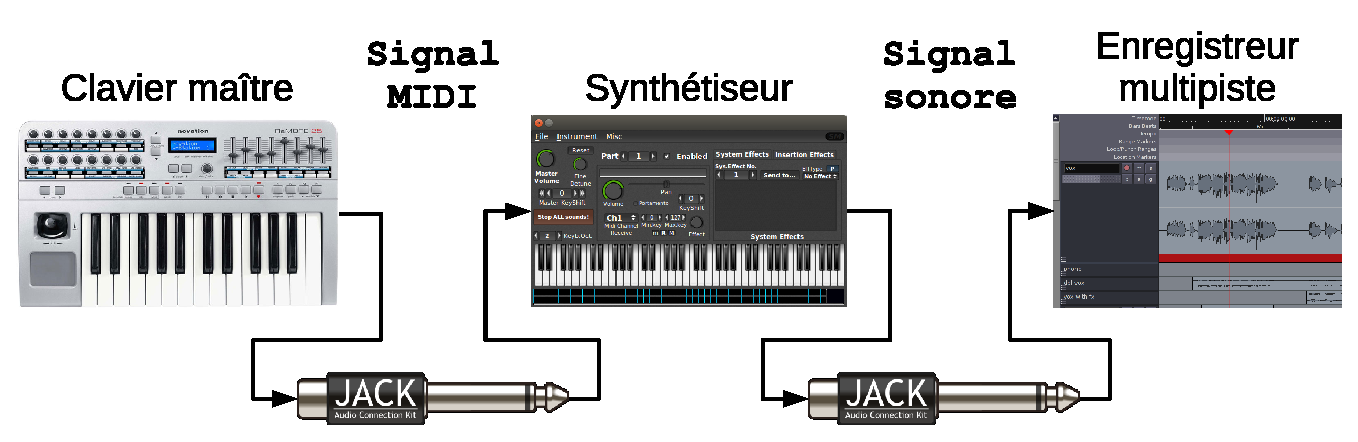
\includegraphics[width=0.8\textwidth]{jack_schema.eps}
  \end{center}
\end{frame}

\begin{frame}{Jack et QJackCtl}
  \textbf{QJackCtl} est l'interface graphique de Jack.
  
  \begin{center}
  %TODO: 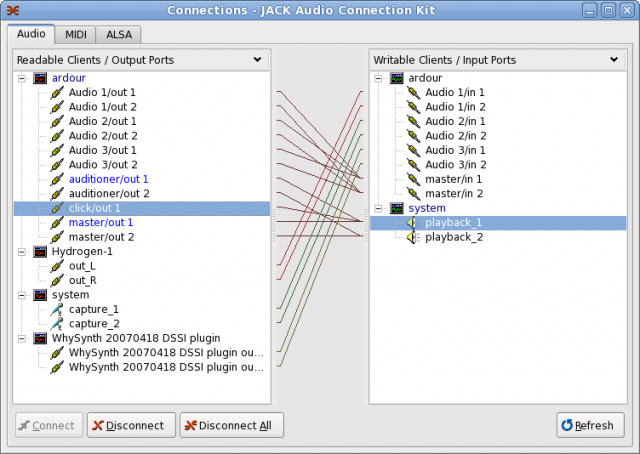
\includegraphics[scale=0.5]{qjackctl_connections.eps}
  \end{center}
\end{frame}

\subsubsection{Ardour}
\begin{frame}{Ardour}
  \begin{columns}
  \begin{column}{0.15\textwidth}
    
\includegraphics[width=\linewidth]{ardour_logo}
  \end{column}
  \begin{column}{0.85\textwidth}
    \textbf{Ardour} est un \textbf{enregistreur multipiste}, ainsi qu'un logiciel de \textbf{montage} et de \textbf{traitement} du son. C'est l'outil principal que nous allons utiliser.

    Très complet, de niveau professionnel.
    Il est \textbf{payant}, mais \textbf{le prix est libre}. Vous pouvez l'acheter pour 1\$ ou pour 1M\$.
  \end{column}
  \end{columns}
  \vskip1em
  
  Avec Ardour, nous allons \textbf{enregistrer} des pistes audio venant :
  \begin{itemize}
  \item du matériel (micros, guitares, etc.) ;
  \item d'autres logiciels (à travers Jack).
  \end{itemize}
  Nous allons \textbf{appliquer des effets} et \textbf{monter} les pistes audio ensemble. Enfin, nous allons \textbf{exporter} le projet en un fichier audio.
\end{frame}

\subsubsection{Hydrogen}
\begin{frame}{Hydrogen}
  \begin{columns}
  \begin{column}{0.15\textwidth}
    
\includegraphics[width=\linewidth]{hydrogen_logo}
  \end{column}
  \begin{column}{0.85\textwidth}
    \textbf{Hydrogen} est un \textbf{échantillonneur} : un logiciel de synthèse sonore à partir d'échantillons réels. En particulier, Hydrogen est spécialisé dans les \textbf{batteries} et autres \textbf{instruments de percussion}. Il possède également un \textbf{séquenceur} intégré qui permet d'écrire des lignes de batteries.
  \end{column}
  \end{columns}
  \vskip1em
    
  Avec Hydrogen, nous allons \textbf{simuler des percussions réelles}.
\end{frame}

\subsubsection{ZynAddSubFX}
\begin{frame}{ZynAddSubFX}
  \begin{columns}
  \begin{column}{0.15\textwidth}
    \def\svgwidth{\linewidth}
    \input{zynaddsubfx_logo.pdf_tex}
  \end{column}
  \begin{column}{0.85\textwidth}
    \textbf{ZynAddSubFX} est un \textbf{synthétiseur} : un logiciel de synthèse sonore, cette fois-ci de manière purement logicielle. Il est très puissant et peut produire une gamme de son très large. Pour les débutants, une large gamme de presets est disponible.
  \end{column}
  \end{columns}
  \vskip1em
  
  Avec ZynAddSubFX, nous allons \textbf{simuler des instruments électroniques}.
  Une utilisation avancée étant compliquée, nous allons nous contenter d'utiliser les presets proposés.
\end{frame}

%TODO: LinuxSampler
%TODO: Rosegarden??? Ou alternative

\end{document}

